\iffalse
\documentclass[journal,12pt,twocolumn]{IEEEtran}
\usepackage{amsmath,amssymb,amsfonts,amsthm}
\usepackage{txfonts}
\usepackage{tkz-euclide}
\usepackage{listings}
\usepackage{gvv}
\usepackage[latin1]{inputenc}
\usepackage{adjustbox}
\usepackage{array}
\usepackage{tabularx}
\usepackage{enumitem}
\usepackage{pgf}
\usepackage{lmodern}
\usepackage{circuitikz}
\usepackage{tikz}
\usepackage{graphicx}


\begin{document}
\bibliographystyle{IEEEtran}

\vspace{3cm}

\title{}
\author{EE23BTECH11054 -  Sai Krishna Shanigarapu$^{*}$
}
\maketitle
\newpage
\bigskip

% \renewcommand{\thefigure}{\theenumi}
% \renewcommand{\thetable}{\theenumi}

\section*{Gate ES 2022}
13. \hspace{2pt}Assuming $s>0$; Laplace transform for $f\brak{x}$ = $\sin\brak{ax}$ is\\
\begin{enumerate}[label=(\Alph*)]
    \item $\frac{a}{s^2+a^2}$\\
    \item $\frac{s}{s^2 + a^2}$\\
    \item $\frac{a}{s^2-a^2}$\\
    \item $\frac{s}{s^2-a^2}$
\end{enumerate}
\hfill(GATE 2022 ES)

\solution
\fi
Assuming $Re\brak{s}>0$\\
Using Table \ref{tab:tab1_2022_es_13_054} and Euler's identity\\
    \begin{align}
        \mathcal{L}\brak{\sin\brak{ax}} &= \mathcal{L}\brak{\frac{e^{jax} - e^{-jax}}{2j}}\\
        &= \frac{\brak{\mathcal{L}\brak{e^{jax}} - \mathcal{L}\brak{e^{-jax}}}}{2j}\\
        &= \frac{2}{2j}\brak{\frac{1}{s-ja}-\frac{1}{s+ja}}\\
        &= \frac{1}{2j}\brak{\frac{2ja}{s^2 + a^2}}\\
        &= \frac{a}{s^2 + a^2}
    \end{align}
\bigskip
    

$\therefore$ Option (A) is correct.

\begin{table}[ht]
       \setlength{\arrayrulewidth}{0.3mm}
\setlength{\tabcolsep}{20pt}
\renewcommand{\arraystretch}{1.3}



\begin{tabular}{|c|c|}
\hline

$y\brak{x}$ & $\mathcal{L}\brak{y\brak{x}}$\\
\hline
$e^{ax}$ & $\frac{1}{s-a}$\\
\hline
$k\, y\brak{x}$ & $k\mathcal{L}\brak{y\brak{x}}$, where k is constant\\
\hline
$y''\brak{x}$ & $s^2\mathcal{L}\brak{y\brak{x}} - sy\brak{0} - y'\brak{0}$\\
\hline
\end{tabular}
    \caption{Laplace transforms}
    \label{tab:tab1_2022_es_13_054}
\end{table}

\begin{figure}[ht]
    \centering
    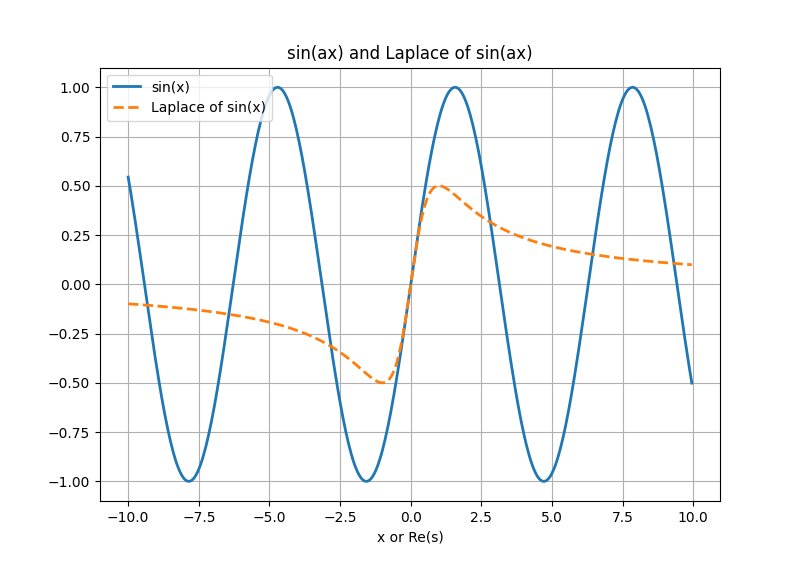
\includegraphics[width=\columnwidth]{2022/ES/13/figs/Figure_1.png}
    \caption{plot of sin(ax) and it's laplace transform}
    \label{fig:fig1_2022_es_13_054}
\end{figure}

\begin{figure}[ht]
    \centering
    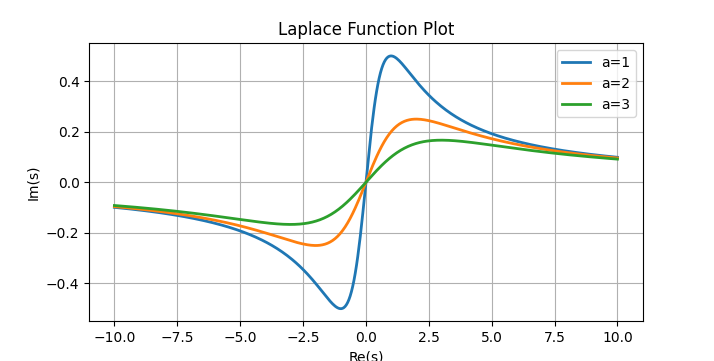
\includegraphics[width=\columnwidth]{2022/ES/13/figs/Figure_2.png}
    \caption{plots of laplace forms of sin(ax)}
    \label{fig:fig2_2022_es_13_054}
\end{figure}

%\end{document}
